\documentclass[crop, tikz]{standalone}
\usepackage{tikz}

\usetikzlibrary{calc}
\usepackage{colortbl}

 
 % Definition of circles
\def\square{(-2,-2) rectangle (4,2)}
\def\firstcircle{(0,0) circle (1.5cm)}
\def\secondcircle{(0:2cm) circle (1.5cm)}

\colorlet{circle edge}{black}
\colorlet{circle area}{gray!30!blue!20}

\colorlet{circle edge2}{black!80}
\colorlet{circle area2}{blue}


\tikzset{filled/.style={fill=circle area, draw=circle edge, thick},
	filled2/.style={fill=circle area2, draw=circle edge2, thick},
    outline/.style={draw=circle edge, thick}}

\setlength{\parskip}{5mm}
 
 \begin{document}
 % not A and not Q
\def\npnq{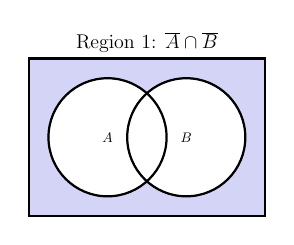
\begin{tikzpicture}[scale=0.5, transform shape]
\begin{scope}
 \draw[filled]   \square;
\end{scope}
\draw[fill=white] \firstcircle;
\draw[fill=white] \secondcircle;
\draw[outline] \firstcircle node  {$A$};
\draw[outline] \secondcircle node  {$B$};
 \draw[outline] \square; 
  \node[anchor=south] at (current bounding box.north) {\Large Region 1: $\overline{A} \cap\overline{B}$};

\end{tikzpicture}
}

\def\pnq{
% A and not Q
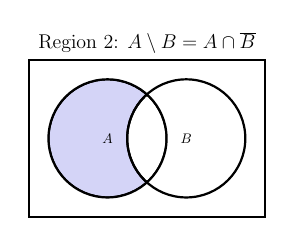
\begin{tikzpicture}[scale=0.5, transform shape]
 \begin{scope}
 \clip \firstcircle;
\draw[filled, even odd rule]  \secondcircle \firstcircle;
\end{scope}
\draw[outline] \firstcircle node  {$A$};
\draw[outline] \secondcircle node  {$B$};
 \draw[outline] \square; 
 \node[anchor=south] at (current bounding box.north) {\Large Region 2:  $A\setminus B = A \cap \overline{B}$};
\end{tikzpicture}
}


\def\pq{
% A and Q
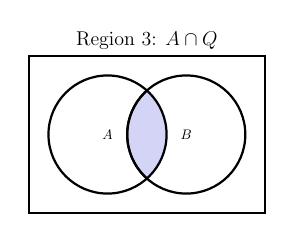
\begin{tikzpicture}[scale=0.5, transform shape]
\begin{scope}
\clip \firstcircle;
 \fill[filled]   \secondcircle;
\end{scope}
\draw[outline] \firstcircle node  {$A$};
\draw[outline] \secondcircle node  {$B$};
 \draw[outline] \square; 
 
 \node[anchor=south] at (current bounding box.north) {\Large Region 3:  $A \cap Q$};

\end{tikzpicture}
}


\def\npq{
% not P and  Q
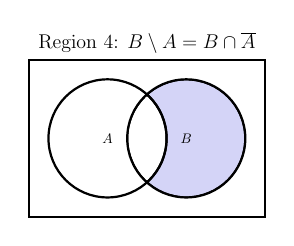
\begin{tikzpicture}[scale=0.5, transform shape]
 \begin{scope}
 \clip \secondcircle;
\draw[filled, even odd rule]  \secondcircle \firstcircle;
\end{scope}
\draw[outline] \firstcircle node  {$A$};
\draw[outline] \secondcircle node  {$B$};
 \draw[outline] \square; 
 
\node[anchor=south] at (current bounding box.north) {\Large Region 4:  $B\setminus A = B\cap \overline{A}$};

\end{tikzpicture}
}

 
\begin{tikzpicture}[scale=1, transform shape] 
 

\node at (-4,0) {\begin{minipage}{1.15in}\npnq\end{minipage}};
\node at (0,0) {\begin{minipage}{1.15in}\pnq\end{minipage}};
\node at (-4,-3) {\begin{minipage}{1.15in}\pq\end{minipage}};
\node at (0,-3) {\begin{minipage}{1.15in}\npq\end{minipage}};


 
 
\end{tikzpicture}
 
\end{document}
